\documentclass[a4paper,12pt]{article}
\usepackage{ucs}
\usepackage[unicode,verbose]{hyperref}
\usepackage{amsmath,amssymb,amsthm}
\usepackage{pb-diagram}
\usepackage{multicol}
\usepackage[utf8x]{inputenc}
\usepackage[russian]{babel}
\usepackage{cmap}
\usepackage{color}
\usepackage[pdftex]{graphicx}
\pagestyle{plain}

%\usepackage{verbatim} 
\newenvironment{comment}
{\par\noindent{\bf TODO}\\}
{\\\hfill$\scriptstyle\blacksquare$\par}

\newtheorem{statement}{Statement}
\theoremstyle{definition} \newtheorem{Def}{Definition}
\newcommand{\go}{\overset{\circ }{\frak{g}}}
\newcommand{\ao}{\overset{\circ }{\frak{a}}}
\newcommand{\co}[1]{\overset{\circ }{#1}}

\begin{document}

\pagenumbering{arabic}
\title{\textbf{{\Large {Recursive algorithms, branching coefficients affine algebras and applications}}}}
\author{Vladimir Lyakhovsky \thanks{ Supported by
 RFFI grant N 09-01-00504 and the National Project RNP.2.1.1./1575 }\\
Theoretical Department, SPb State University,\\
198904, Sankt-Petersburg, Russia \\
e-mail:lyakh1507@nm.ru \\
[5mm] Anton Nazarov \thanks{ Supported by
the National Project RNP.2.1.1./1575 }\\
Theoretical Department, SPb State University,\\
198904, Sankt-Petersburg, Russia \\
e-mail:antonnaz@gmail.com
}
\maketitle

\begin{abstract}
Примерный текст доклада на семинаре кафедры ФВЭиЭЧ по работе ``Recursive algorithms, branching coefficients and applications''.
\end{abstract}

\section{Постановка задачи}
\label{sec:task}

Здравствуйте!
Сегодня я хочу рассказать о работе ``Рекуррентные алгоритмы, коэффициенты ветвления аффинных алгебр
Ли и приложения''. В этой работе мы решали следующую задачу.

Даны две аффинные алгебры Ли $\mathfrak{a}\subset \mathfrak{g}$. Неприводимое представление
$L^{(\mu)}_{\mathfrak{g}}$ алгебры $\mathfrak{g}$ со старшим весом $\mu$ может быть разложено на
представления подалгебры $\mathfrak{a}$. Наша задача --- придумать практический алгоритм вычисления
коэффициентов этого разложения. Конечно же эта задача уже решалась, существует способ решения ``в лоб'', требующий построения всех представлений и различные способы, которые работают для частных случаев, например, многое упрощается в физически интересном случае конформных вложений. Мы предлагаем общий метод, но иллюстрировать его будем физическими примерами (которые можно вычислять и другими способами).

Я начну с физической мотивации этой задачи в двумерной конформной теории поля, напомню некоторые
факты из теории представлений аффинных алгебр Ли, кратко опишу предложенное нами решение проблемы и
расскажу про физические примеры в нашей статье.

\section{Физическая мотивация}
\label{sec:physics}

\subsection{Напоминание про двумерную конформную теорию поля}
\label{sec:CFT}

В теории струн двумерная конформная теория поля описывает динамику на мировой поверхности, а в
теории критических явлений --- фазовые переходы в двумерных системах.

Конформное преобразование --- это преобразование, меняющее только масштаб у метрического тензора:
\begin{equation}
  \label{eq:10}
  g'_{\mu\nu}(x')=\Lambda(x)g_{\mu\nu}(x)
\end{equation}

Конформная теория поля --- это теория поля, обладающая инвариантностью относительно этих преобразований.

%% В $D$-мерном случае генераторы у таких преобразований следующие:
%% \begin{align}
%%   \label{eq:1}
%%   & M_{\mu\nu} \equiv i(x_\mu\partial_\nu-x_\nu\partial_\mu) \,, \\
%%   &P_\mu \equiv-i\partial_\mu \,, \\
%%   &D \equiv-ix_\mu\partial^\mu \,, \\
%%   &K_\mu \equiv i(x^2\partial_\mu-2x_\mu x_\nu\partial^\nu) \,,
%% \end{align}
%% 
На двумерной мировой поверхности удобно ввести комплексные координаты $z,\bar{z}$. 
В двумерном случае существует бесконечное число локально-конформных преобразований.
Это легко можно увидеть из условия конформности преобразований, так как в двумерном случае это условие эквивалентно уравнению Коши-Римана для голоморфных функций ($\partial_{\bar z}w(z,\bar z)=0$).

В этом случае конформная группа --- это набор всех аналитических функций $w(z)$ на плоскости. 

Для классической теории алгебра конформных преобразований --- это алгебра Витта, которая порождается
генераторами $\{L_n, n\in \mathbb{Z}\}$ --- модами разложения оператора энергии-импульса $T$, с
коммутационными соотношениями
\begin{equation}
  \label{eq:2}
  [L_m,L_n]=(m-n)L_{m+n}
\end{equation}
При квантовании возникает конформная аномалия, что соответствует центральному расширению алгебры (то
есть появлению центрального заряда $c$). В коммутационные соотношения надо добавить член
$\frac{c}{12}(m^3-m)\delta_{m+n,0}$. В результате получаем алгебру Вирасоро.
В двумерной конформной теории поля тензор энергии-импульса бесследовый.

Поля теории $\phi(z,\bar z)$ должны преобразовываться определенным образом при конформных преобразованиях.
Оказывается, что все поля группируются в конформные семейства, в которых есть одно примарное поле
\begin{equation}
  \label{eq:3}
  \begin{split}
    \phi_{\Delta,\bar \Delta}(z,\bar z)\underset{
      \genfrac{}{}{0pt}{}{z\to w(z)}
        {\bar z \to \bar w(\bar z)}
    }
    {\longrightarrow} \left(\frac{dw}{dz}\right)^{\Delta}\left(\frac{d\bar w}{d\bar
        z}\right)^{\bar\Delta}\phi_{\Delta,\bar \Delta}(w(z),\bar w(\bar z))\\
    L_n \phi=0,\quad n>0\\
    L_0 \phi=\Delta \phi\\
  \end{split}
\end{equation}
$\Delta, \bar \Delta$ называются конформными размерностями поля.
Все остальные поля называются вторичными и получаются из примарного действием операторов $L_{-n}$:
\begin{equation}
  \label{eq:67}
  L_{-n_1}L_{-n_2}\dots \phi_{\Delta}
\end{equation}
Все поля в теории оказываются суммами мультиплетов алгебры Вирасоро.

При некоторых дополнительных предположениях двумерную конформную теорию можно построить и решить
полностью, если определен набор примарных полей и аномальных размерностей. 

Существуют различные подходы к аксиоматизации двумерной конформной теории поля. В общем случае нам
не нужно знать действие, если мы полный знаем набор примарных полей и операторные разложения их
произведений. 

В том случае, если в теории конечное число примарных полей, такая теория называется минимальной.
Кроме того, теории классифицируются по значениям центрального заряда $c$. Теории с рациональным
центральным зарядом называются рациональными. Оказывается, что все такие теории могут быть получены
факторизацией так называемых моделей Весса-Зумино-Новикова-Виттена.

\subsection{WZW-модели}
\label{sec:wzw}

WZW-модели обладают дополнительной симметрией. Алгебра токов в них --- это алгебра Каца-Муди
(аффинная алгебра Ли $\mathfrak{g}$), а полная киральная алгебра --- полупрямое произведение
$Vir\ltimes \mathfrak{g}$. 

Сейчас я поясню, что все это значит и как строятся такие модели.

Модели Весса-Зумино-Виттена можно строить начиная со следующего действия:
\begin{equation}
\label{eq:4}
  S=S_0+k\Gamma
\end{equation}
где $k$ - целое.
Здесь $S_0$ --- действие нелинейной $\sigma$-модели.
\begin{equation}
  \label{eq:5}
  S_0=\frac{1}{4a^2}\int_{\partial B} d^2x\; Tr (\partial^{\mu}g^{-1}\partial_{\mu}g),
\end{equation}
где $a^2>0$ - положительный параметр, $g(x)\in G$ - поле со значениями в группе $G$, которую мы
будем считать полупростой. 

В нелинейной $\sigma$-модели конформная инвариантность теряется на квантовом уровне.
Голоморфный и антиголоморфный токи не сохраняются по отдельности.
Поэтому мы добавляем член Весса-Зумино $\Gamma$ к действию
\begin{equation}
  \label{eq:73}
\Gamma= - \frac{i }{24\pi} \int_{B}\epsilon_{ijk} Tr\left(
    \tilde g^{-1}\frac{\partial \tilde g}{\partial y^i}
      \tilde g^{-1}\frac{\partial \tilde g}{\partial y^j}
      \tilde g^{-1}\frac{\partial \tilde g}{\partial y^k}\right) d^3y
\end{equation}
Он определен на трехмерном многообразии $B$, ограниченном исходным двумерным пространством.
Через $\tilde{g}$ мы обозначили продолжение поля $g$ на $B$. Такое продолжение не единственно. В
компактифицированном трехмерном пространстве компактное двумерное многообразие разделяет два
трехмерных многообразия. Разность значений члена Весса-Зумино $\Delta\Gamma$ на этих многообразиях
дается правой частью уравнения (\ref{eq:73}) с интегралом, продолженным на все компактное трехмерное
пространство. Так как оно топологически эквивалентно три-сфере, получаем
\begin{equation}
  \label{eq:75} \Delta\Gamma= - \frac{i }{24\pi} \int_{S^3}\epsilon_{ijk} Tr'\left( \tilde
g^{-1}\frac{\partial \tilde g}{\partial y^i} \tilde g^{-1}\frac{\partial \tilde g}{\partial y^j}
\tilde g^{-1}\frac{\partial \tilde g}{\partial y^k}\right) d^3y
\end{equation}
$\Delta\Gamma$ определен по модулю $2\pi i$, поэтому Евклидов функциональный интеграл
с весом $exp(-\Gamma)$ хорошо определен. Значит константа связи, умножаемая на этот член, должна
быть целочисленной.

Уравнение движения для полного действия (\ref{eq:4}):
\begin{equation}
  \label{eq:77}
  \partial^{\mu}(g^{-1}\partial_{\mu}g)+\frac{a^2 ik}{4\pi}\epsilon_{\mu\nu}\partial^{\mu}(g^{-1}\partial^{\nu}g)=0
\end{equation}
В комплексных координатах оно записывается в виде
\begin{equation}
  \label{eq:78}
  (1+\frac{a^2 k}{4\pi})\partial_z(g^{-1}\partial_{\bar z}g)+(1-\frac{a^2 k}{4\pi})\partial_{\bar z}(g^{-1}\partial_z g)=0
\end{equation}
Видно, что при $a^2=\frac{4\pi}{k}$ у нас имеются законы сохранения
\begin{equation}
  \label{eq:79}
  \partial_z(g^{-1}\partial{\bar z}g)=0
\end{equation}
Для токов
\begin{equation}
  \label{eq:72}
  J_z=\partial_z g\;g^{-1}, \qquad J_{\bar{z}}=g^{-1}\partial{\bar z}g
\end{equation}

\begin{equation}
  \label{eq:100}
  \partial_{\bar z}J=0,\quad \partial_z \bar J=0
\end{equation}
То есть голоморфная и антиголоморфная части отщепляются, что является указанием на наличие
конформной инвариантности.

Решение классического уравнения движения имеет вид
\begin{equation}
  \label{eq:80}
  g(z,\bar z)=f(z)\bar f(\bar z)
\end{equation}
при произвольных $f(z)$ и $\bar f (\bar z)$.

Сохранение по отдельности токов $J_z,\; J_{\bar z}$ приводит к инвариантности действия при преобразованиях
\begin{equation}
  \label{eq:81}
   g(z,\bar z)\to \Omega(z)g(z,\bar z)\bar \Omega^{-1}(\bar z)
\end{equation}
где $\Omega,\;\bar \Omega \in G$. То есть мы получили локальную $G(z)\times G(\bar z)$-инвариантность.

Для перехода к квантовому случаю мы переопределяем токи
\begin{equation}
  \label{eq:82}
  J(z)\equiv -k \partial_zg g^{-1}\quad \bar J(\bar z)=k g^{-1}\partial_{\bar z}g
\end{equation}
Тогда вариация действия при инфинитезимальных преобразованиях $\Omega=1+\omega,\; \bar \Omega =1+\bar \omega$ дается выражением
\begin{equation}
  \label{eq:83}
  \delta_{\omega,\bar\omega}S=\frac{i}{4\pi}\oint dz Tr (\omega(z)J(z))-\frac{i}{4\pi}\oint d\bar z Tr(\bar\omega(\bar z)\bar J(\bar z))
\end{equation}
Раскладывая токи
\begin{equation}
  \label{eq:85}
  \begin{aligned}
    J=\sum J^a t^a,\bar J=\sum \bar J^a t^a \\
    \omega=\sum \omega^a t^a\\
  \end{aligned}
\end{equation}
получаем
\begin{equation}
  \label{eq:86}
  \delta_{\omega,\bar \omega}S=-\frac{1}{2\pi i}\oint dz \sum\omega^a J^a+\frac{1}{2\pi i} \oint d\bar z \sum \bar \omega^a \bar J^a
\end{equation}
Мы также получили тождества Уорда $\delta\left< X\right>=\left<(\delta S)X\right>$
\begin{equation}
  \label{eq:87}
  \delta_{\omega,\bar \omega}\left< X \right>=-\frac{1}{2\pi i}\oint dz \sum\omega^a \left< J^a X\right>+
  \frac{1}{2\pi i} \oint d\bar z \sum \bar \omega^a \left< \bar J^a X\right>
\end{equation}
Для токов имеем
\begin{equation}
  \label{eq:88}
  \delta_{\omega}J=[\omega,J]-k\partial_z\omega,\quad \delta_{\omega}J^a=\sum i f_{abc}\omega^b J^c-k\partial_z\omega^a
\end{equation}
Операторное разложение для токов имеет вид
\begin{equation}
  \label{eq:89}
  J^a(z) J^b(w) \sim \frac{k\delta_{ab}}{(z-w)^2}+\sum i f_{abc}\frac{J^c(w)}{(z-w)}
\end{equation}
Раскладывая токи в ряд, получаем
\begin{equation}
  \label{eq:90}
  \begin{aligned}
    J^a(z)=\sum_{n\in \mathbb Z}z^{n-1}J^a_n\\
    \left[J^a_n,J^b_m\right]=\sum_c i f^{abc}J^c_{n+m}+kn\delta^{ab}\delta_{n+m,0}
  \end{aligned}
\end{equation}
Теперь мы видим, что компоненты токов образуют аффинную алгебру Ли $\hat g$.


Тензор энергии-импульса вводится при помощи конструкции Сугавары как сумма нормально упорядоченных компонент токов
\begin{equation}
  \label{eq:102}
  T(z)=\frac{1}{2(k+h^v)}\sum_a N(J^a J^a)(z)
\end{equation}
Здесь $h^v$ - дуальное число Кокстера.

Тензор энергии-импульса можно разложить на моды $L_n$
\begin{equation}
  \label{eq:91}
  L_n=\frac{1}{2(k+h^v)}\sum_a\sum_m:J^a_m J^a_{n-m}:
\end{equation}
Тогда коммутационные соотношения для мод $L_n$ имеют вид
\begin{equation}
  \label{eq:92}
  \begin{aligned}
    \left[L_n,L_m\right]=(n-m)L_{n+m}+\frac{c}{12}(n^3-n)\delta_{n+m,0}\\
    \left[L_n,J^a_m\right]=-mJ^a_{n+m}
  \end{aligned}
\end{equation}

Таким образом, конструкция Сугавары --- это способ вложения алгебры Вирасоро в универсальную обертывающую аффинной алгебры Ли $\hat{g}$

Полная киральная алгебра модели Весса-Зумино-Виттена равна полупрямому произведению $Vir\ltimes \hat g$

Примарными оказываются поля, которые преобразуются ковариантно под действием $G(z)\times G(\bar z)$,
как $g(z,\bar z)$. В терминах операторного разложения это свойство переформулируется следующим
образом:
\begin{equation}
  \label{eq:84}
  \begin{aligned}
    J^a(z)g(w,\bar w)\sim \frac{-t^a g(w,\bar w)}{(z-w)}\\
    \bar J^a(z)g(w,\bar w)\sim \frac{ g(w,\bar w)t^a}{(z-w)}
  \end{aligned}
\end{equation}
Любое поле $\phi_{\lambda,\mu}$, преобразующееся ковариантно по отношению к некоторому
представлению, заданному весом $\lambda$ в голоморфном секторе и весом $\mu$ в антиголоморфном,
является примарным полем WZW-модели.

В модах это свойство записывается в виде
\begin{equation}
  \label{eq:93}
  \begin{aligned}
    & (J_0^a \phi_{\lambda})=-t^a_{\lambda}\phi_{\lambda}\\
    & (J^a_n\phi_{\lambda})=0\quad \mbox{для}\; n>0\\
  \end{aligned}
\end{equation}
Мы можем сопоставить состояние $\left|\phi_{\lambda}\right>$ полю $\phi_{\lambda}$
  \begin{equation}
    \label{eq:94}
    \phi_{\lambda}(0)=\left|\phi_{\lambda}\right>
  \end{equation}
Тогда условия (\ref{eq:93}) для примарных полей дают
\begin{equation}
  \label{eq:95}
  \begin{aligned}
    & J_0^a\left|\phi_{\lambda}\right>=-t^a_{\lambda}\left|\phi_{\lambda}\right>\\
    & J^a_n\left|\phi_{\lambda}\right>=0 \quad \mbox{для}\; n>0 \\
  \end{aligned}
\end{equation}
Легко видеть, что действие генераторов алгебры Вирасоро имеет вид
\begin{equation}
  \label{eq:96}
  L_0\left|\phi_{\lambda}\right>=\frac{1}{2(k+h^v)}\sum_aJ^a_0J^a_0\left|\phi_{\lambda}\right>=\frac{(\lambda,\lambda+2\rho)}{2(k+h^v)}\left|\phi_{\lambda}\right>
\end{equation}
Здесь использовано явное выражение для собственных значений квадратичного оператора Казимира.

Примарные поля живут в интегрируемых конечномерных представлениях, так как бесконечномерные и
неинтегрируемые поля отщепляются в корреляционных функциях.

Все вторичные состояния имеют вид
\begin{equation}
  \label{eq:97}
  J^{a_1}_{-n_1}J^{a_2}_{n_2}\dots\left|\phi_{\lambda}\right>
\end{equation}

\subsection{Конформные вложения и модулярно-инвариантные статсуммы}
\label{sec:modular-invariance}

Если мы изучаем конформную теорию поля на плоскости или на сфере, то мы можем рассматривать
голоморфный и антиголоморфный сектора независимо. В WZW-моделях примарные поля
принадлежат тензорному произведению неприводимых представлений аффинной алгебры.

Если мы говорим о применении конформной теории для описания поведения струн, то теория должна быть
определена на римановых поверхностях большего рода ($h>0$), чтобы можно было описывать
взаимодействия струн. Считается, что для этого необходимо (и, возможно, достаточно) чтобы теория была определена на торе.

В теории критического поведения конформная инвариантность имеет место только в критической точке,
где голоморфный и антиголоморфный сектора расцеплены. Но вблизи критической точки эти сектора должны
быть связаны, и так как мы предполагаем плавный переход к критической точке в пространстве
параметров, то эта связь должна сохраняться и в критической точке. Физический спектр теории должен
плавно меняться, когда мы покидаем критическую точку, и связь голоморфного и антиголоморфного
сектора вдали от критической точки должна приводить к ограничениям на набор состояний в критической
точке. Этого можно достичь через геометрию, то есть накладывая граничные условия на состояния. Здесь
естественно рассматривать периодические граничные условия, которые эквивалентны рассмотрению теории
на торе.

%% Наложим периодические граничные условия с периодами $\omega_1, \omega_2,\; \tau=\omega_2/\omega_1$. 
%% Мы хотим вычислить статсумму для теории на торе через генераторы алгебры Вирасоро $L_0,\bar L_0$ и
%% выяснить ее зависимость от параметра $\tau$. Пусть пространственное направление соответствует
%% вещественной оси, а временное - мнимой. Пусть $\omega_1$ направлен вдоль вещественной оси. Через $H$
%% обозначим гамильтониан, а через $P$ - общий импульс системы. Тогда оператор трансляции на $a$
%% параллельно периоду $\omega_2$ имеет вид $\exp(-\frac{a}{|\omega_2|}(H \mathrm{Im} \omega_2-i P \mathrm{Re} \omega_2))$. 
%% Если считать, что $a$ - расстояние в решетке, то такой сдвиг переводит нас с одного ряда на другой
%% параллельно периоду $\omega_2$. Если полный период содержит $m$ ячеек решетки ($|\omega_2|=ma$), то
%% статсумма дается следом оператора сдвига в степени $m$:
%% \begin{equation}
%%   \label{eq:6}
%%   Z(\omega_1,\omega_2)=\mathrm{Tr} \exp-\{H \mathrm{Im} \omega_2-iP\mathrm{Re}\omega_2\}
%% \end{equation}
%% Операторы $H,P$ можно выразить через генераторы алгебры Вирасоро если рассмотреть тор как цилиндр
%% конечной длины со склеенными концами. На цилиндре с длиной окружности $L$ гамильтониан
%% $H=(2\pi/L)(L_0+\bar L_0-c/12)$. Константа добавлена, чтобы вакуумная энергия исчезала в пределе
%% $L\to \infty$. Оператор импульса, который генерирует трансляции вокруг окружности, имеет вид
%% $P=(2\pi i/L)(L_0-\bar L_0)$. Так как мы выбрали $\omega_1$ вещественным и равным $L$, статсумму
%% можно записать в виде
%% \begin{equation}
%%   \label{eq:7}
%%   \begin{split}
%%       Z(\tau)=\mathrm{Tr}\exp \pi i \{(\tau-\bar \tau)(L_0+\bar L_0-c/12)+(\tau+\bar \tau)(L_0-\bar
%%       L_0)\}\\
%%       =\mathrm{Tr} \exp 2 \pi i \{\tau(L_0-c/24)-\bar\tau (\bar L_0-c/24)\}\\
%%   \end{split}
%% \end{equation}
%% Или, если ввести $q=\exp 2\pi i \tau$
%% \begin{equation}
%%   \label{eq:2}
%%   Z(\tau)=Tr \left (q^{L_0-c/24}\bar{q}^{\bar{L}_0-c/24}\right)
%% \end{equation}
%% Это выражение, на самом деле --- сумма характеров представлений алгебры Вирасоро (конформных семейств).
%% 
%% Двумерный тор представляет собой фактор пространство $\mathbb{R}^2\approx \mathbb{C}$ по отношениям
%% эквивалентности $z\sim z+w_1$ and $z\sim z+w_2$, где $w_1$ и $w_2$ не параллельны.
%% 
Разные параметризации тора связаны модулярными преобразованиями, таким образом возникает требование
модулярной инвариантности статсуммы.

Комплексная структура тора конформно эквивалентна тору, для которого соотношения
эквивалентности записываются в виде $z\sim z+1$ и $z\sim z+\tau$, где $\tau$ в верхней полуплоскости
$\mathbb{C}$.
%% 
%% Легко видеть, что $\tau$, $T(\tau)=\tau+1$ и $S(\tau)=-\frac{1}{\tau}$ описывают
%% конформно-эквивалентные торы. Отображения $T$ и $S$ порождают группу
%% $SL(2,\mathbb{Z})/\mathbb{Z}_2$, состоящую из матриц вида
%% \begin{equation}
%%   \label{eq:99} A=
%%   \begin{pmatrix} a & b\\ c & d
%%   \end{pmatrix} \quad\mbox{где}\; a,b,c,d\in\mathbb{Z},\quad ad-bc=1,
%% \end{equation}
%% и матрицы $A$ и $-A$ действуют одинаково на $\tau$
%% \begin{equation}
%%   \label{eq:100} \tau\to A\tau=\frac{a\tau+b}{c\tau+d}
%% \end{equation}
%% $\tau$ называется модулярным параметром, а группа $SL(2,\mathbb{Z})/\mathbb{Z}_2$ ---
%% модулярной группой.
%% 
Конформная теория поля задаётся примарными полями $\Phi_a$ с конформными размерностями $\Delta_a$:
\begin{equation}
  \label{eq:3}
  \begin{split} \Phi_{a}(z)\underset{z\to w(z)}{\longrightarrow}
\left(\frac{dw}{dz}\right)^{\Delta_a}\Phi_{a}(w(z))\\ L_n \Phi_a=0,\quad n>0\\ L_0 \Phi_a=\Delta_a
\Phi_a\\
  \end{split}
\end{equation}

Примарные поля живут в пространствах $\mathcal{H}_{(i,j)}$, которые представляют собой тензорные
произведения неприводимого представления $\mathcal{H}_j$ киральной алгебры и неприводимого
представления $\bar{\mathcal{H}}_{\bar{j}}$ антикиральной алгебры. Тогда статсуммы на торе
(\ref{eq:2}) может быть записана в виде
\begin{equation}
  \label{eq:9}
    Z(\tau)=\sum_{(j,\bar j)}\chi_j(q)\bar \chi_{\bar j}(\bar q)
\end{equation}
где $\chi_j$ --- характер представления $\mathcal{H}_j$,
\begin{equation}
  \label{eq:5} \chi_j(\tau)=Tr_{\mathcal{H}_j}(q^{L_0-\frac{c}{24}})\quad \mbox{где}\; q=e^{2\pi i
\tau}
\end{equation}
Характеры переходят друг в друга при модулярных преобразованиях:
\begin{equation}
  \label{eq:107} \chi_j\left(-\frac{1}{\tau}\right)=\sum_k S_{jk}\chi_k(\tau)\quad \mbox{и}\quad
\chi_j(\tau+1)=\sum_kT_{jk}\chi_k(\tau),
\end{equation}
где $S$ и $T$ --- постоянные матрицы. Это верно для большого класса конформных теорий
поля.

Для WZW-моделей примарные поля определяются старшими весами  $\hat \lambda, \hat \xi$ соответствующих представлений алгебры $\mathfrak{g}$. Тогда
\begin{equation}
  \label{eq:6} \mathcal{H}=\bigoplus_{\hat \lambda,\hat \xi\in P^{(k)}_{+}}M_{\hat \lambda,\hat \xi}
L_{\hat \lambda}\otimes L_{\hat \xi}
\end{equation}

Коэффициенты ветвления для вложения аффинной подалгебры Ли в аффинную алгебру можно использовать для
построения модулярно-инвариантной статсуммы в соответствующей WZW-модели. Когда рассматривается
теория на торе,  набор физически допустимых полей ограничен требованиями модулярной инвариантности.

Простейший модулярный инвариант можно записать следующим образом:
\begin{equation}
  \label{eq:34}
   Z(\tau)=\sum_{ \mu\in P^{+}_{\mathfrak{g}}} \chi_{\mu}(\tau)\bar \chi_{\mu}(\bar \tau)
\end{equation}
Здесь суммирование ведется по всем конформным семействам (то есть по всем представлениям алгебры
$\mathfrak{g}$).

Другие модулярные инварианты в WZW-модели с алгеброй $\mathfrak{a}$ можно получить, если существует алгебра $\mathfrak{g}$, в которую $\mathfrak{a}$ вкладывается конформно. (Я сейчас поясню, что это значит).

Представления алгебры можно рассматривать как сумму представлений подалгебры. 

Если мы рассмотрим редукцию характеров
\begin{equation}
  \label{eq:8}
   \pi_{\mathfrak{a}}(ch L^{\mu}_{\mathfrak{g}})=
  \sum_{\nu\in P^{+}_{\mathfrak{a}}}b^{(\mu)}_{\nu} ch L^{\nu}_{\mathfrak{a}}
\end{equation}
и подставим разложение в формулу \eqref{eq:34}, то модулярная инвариантность сохранится. То есть из диагонального инварианта для алгебры $\mathfrak{g}$ мы получаем новый не диагональный инвариант для подалгебры $\mathfrak{a}$. 
Но возникает вопрос, будет ли теория, полученная таким образом, самосогласованной, сохранится ли в
ней конформная инвариантность.

Для этого требуется, чтобы вложение подалгебры было ``конформным'', то есть центральные заряды
теорий должны совпадать.
\begin{equation}
  \label{eq:31}
  c(\mathfrak{a})=c(\mathfrak{g})
\end{equation}

Пусть $X^{a_j}_{-n_j}$ и $\tilde{X}^{a'_j}_{-n_j}$ --- понижающие операторы алгебр  $\mathfrak{g}$ и
$\mathfrak{a}\subset\mathfrak{g}$.  $\pi_{\mathfrak{a}}$ --- проекционный оператор
$\pi_{\mathfrak{a}}:\mathfrak{g}\longrightarrow \mathfrak{a}$. В теории, связанной с  $\mathfrak{g}$
с вакуумом $\left|\lambda\right>$ будут следующие состояния:
\begin{equation}
  \label{eq:109}
  X^{a_1}_{-n_1}X^{a_2}_{-n_2}\dots\left|\lambda\right>\quad n_1\geq n_2\geq \dots>0.
\end{equation}
Вакуум $\mathfrak{g}$-инвариантен, то есть $X_0^a\left|0\right>=0$. При проекции на подалгебру
$\mathfrak{a}$ состояния примут вид
\begin{equation}
  \label{eq:110}
  \tilde{X}^{a'_1}_{-n_1}\tilde{X}^{a'_2}_{-n_2}\dots\left|\pi_{\mathfrak{a}}(\lambda)\right>.
\end{equation}
Из $\mathfrak{g}$-ивариантности вакуума следует его $\mathfrak{a}$-инвариантность, но для тензора
энергии-импульса в общем случае это не так. Поэтому тензор энергии-импульса большей теории должен
состоять только из генераторов $\tilde{X}$. Тогда $T_{\mathfrak{g}}=T_{\mathfrak{a}}\Rightarrow
c(\mathfrak{g})=c(\mathfrak{a})$. Это приводит к уравнению
\begin{equation}
  \label{eq:111}
  \frac{k\;\mathrm{dim}\,\mathfrak{g}}{k+g}=\frac{x_e k\; \mathrm{dim}\,\mathfrak{a}}{x_ek+a}
\end{equation}
Здесь $x_e$ --- индекс вложения, а  $g$, $a$ --- дуальные числа Кокстера, которые характеризуют алгебры.

Можно показать, что только для представлений уровня 1 это равенство удовлетворяется. То есть класс
конформных вложений не слишком широк и существует полная их классификация. Кроме того, для
конформных вложений существуют специальные методы разложения представлений.

Модулярная инвариантность статсуммы для полей, принадлежащих представлениям алгебры  $\mathfrak{g}$,
сохраняется при проекции на подалгебру $\mathfrak{a}$. Если все представления $\mathfrak{g}$ в теории
удовлетворяют описанным требованиям, то при проекции мы получаем конформную теорию поля.

Существует теорема о том, что для конформного вложения  $\mathfrak{a}\subset\mathfrak{g}$ только
конечное число коэффициентов ветвления отлично от нуля. Поэтому после того, как мы разложили все
представления $\mathfrak{g}$ мы подставляем результаты в выражение для статсуммы и получаем
модулярно-инвариантную статсумму для вложенной теории. Такая статсумма уже не будет иметь
диагональный вид:
\begin{equation}
  \label{eq:36}
   Z_{\mathfrak{a}}(\tau)=\sum_{ \nu,\lambda\in P^{+}_{\mathfrak{a}}} \chi_{\nu}(\tau)M_{\nu\lambda}\bar \chi_{\lambda}(\bar \tau)
\end{equation}
Наша работа посвящена разработке общего метода редукции представлений аффинных алгебр Ли, поэтому
случай конформных вложений --- лишь один из примеров применения нашего метода. Однако в этом случае
физический смысл наиболее очевиден. 

Теперь я перейду к краткому объяснению метода и примерам вычислений.

\section{Рекуррентные соотношения для коэффициентов ветвления}
\label{sec:branching}

Ранее для вычисления коэффициентов ветвления был предложен способ, основанный на преобразовании
формулы Вейля-Каца для характеров представлений аффинных алгебр Ли в рекуррентное соотношение для
коэффициентов ветвления. Однако исходный алгоритм не работал для не максимальных вложений. В данной
работе была решена данная проблема и предложено обобщение рекуррентных соотношений на данный случай. 

Общая идея метода в следующем:




В результате рекуррентные соотношения имеют вид
\begin{equation}
  \label{eq:1}
  \begin{array}{c}
      k_{\xi }^{\left( \mu \right) }=-\frac{1}{s\left( \gamma _{0}\right) }\left(
  \sum_{\omega\in W_{\bot}\backslash W} \epsilon(\omega)\; {\rm dim}\left(L^{\pi_{\mathfrak{a}_{\bot}}(\omega(\mu+\rho))-\rho_{\mathfrak{a}_{\bot}}}_{\mathfrak{a}_{\bot}}\right) \delta_{\xi-\gamma_0,\pi_{\mathfrak{a}}(\omega(\mu+\rho)-\rho)}+ \right.\\
\left.
+\sum_{\gamma \in
\Gamma _{\frak{a}\subset \frak{g}}}s\left( \gamma +\gamma _{0}\right) k_{\xi
+\gamma }^{\left( \mu \right) }\right)
  \end{array}
\end{equation}
Здесь $\mathfrak{a}_{\bot}$ --- это подалгебра, ``натянутая'' на корни $\mathfrak{g}$, ортогональные
к корневой системе подалгебры  $\mathfrak{a}$, $W_{\bot}$ --- соответствующая этим корням группа Вейля,
$\Gamma_{\mathfrak{a}\subset \mathfrak{g}}$ --- набор весов в разложении знаменателя $\prod_{\alpha\in \Delta^{+}\setminus \Delta^{+}_{\mathfrak{a}_{\bot}}}
(1-e^{-\alpha})^{\mathrm{mult}(\alpha)-\mathrm{mult}_{\mathfrak{a}}(\alpha)}$, а $s(\gamma)$ ---
коэффициент при  $e^{\gamma}$ в этом разложении.

Это рекуррентное соотношение позволяет нам сформулировать следующий алгоритм вычисления
коэффициентов ветвления, который осуществляется без явного построения исходного представления или
представлений, входящих в разложение.
\begin{enumerate}
\item Построить наборы положительных корней $\Delta^{+}$ и $\Delta_{\mathfrak{a}}^{+}$.
\item Выбрать те положительные корни $\alpha\in \Delta^{+}$, которые ортогональны корневому
  подпространству  $\mathfrak{a}$ и собрать их в набор $\Delta^{+}_{\bot}$.
\item Построить множество весов $\Gamma$, которое мы называем ``веером''.
\item Найти множество $\widehat{\Psi^{(\mu)}}=\left\{\omega(\mu+\rho)-\rho;\; \omega\in W\right\}$
  аномальных весов представления $L^{(\mu)}_{\mathfrak{g}}$.
\item Выбрать в нем веса $\left\{ \lambda=\omega(\mu+\rho) | \pi_{\mathfrak{a}_{\bot}}\lambda \in
    \bar{C}_{\mathfrak{a}_{\bot}} \right\}$. Это можно легко сделать, так как у нас есть набор
  $\Delta^{+}_{\bot}$ и мы можем проверить, лежит ли вес $\pi_{\mathfrak{a}_{\bot}}\lambda$ в
  главной камере Вейля алгебры $\mathfrak{a}_{\bot}$. Для этого все скалярные произведения этого
  веса $\lambda$ с корнями из  $\Delta^{+}_{\bot}$ должны быть неотрицательны.
\item Далее для весов $\lambda=\omega(\mu+\rho),\; \pi_{\mathfrak{a}_{\bot}}\lambda\in
  \bar{C}_{\mathfrak{a}_{\bot}}$ мы вычисляем размерность соответствующих представлений
  $\mathrm{dim}\left(L^{\pi_{\mathfrak{a}_{\bot}}(\omega(\mu+\rho))-\rho_{\mathfrak{a}_{\bot}}}_{\mathfrak{a}_{\bot}}\right)$
  при помощи формулы Вейля и набора $\Delta^{+}_{\bot}$.
\item Далее рекуррентно вычисляются аномальные коэффициенты ветвления, а внутри главной камеры Вейля
  алгебры $\mathfrak{a}$ аномальные коэффициенты совпадают с настоящими коэффициентами ветвления.
\end{enumerate}

\subsection{Примеры}
\label{sec:examples}

Я начну с примера вычисления в случае конечномерных простых алгебр Ли, так как его легко нарисовать.

Рассмотрим регулярное вложение  $A_1$ в $B_2$. Вот на рисунке корневая системы алгебры $B_2=so(5)$.
Корень  $\beta$ вложенной алгебры $A_1$ равен $\alpha_1+2\alpha_2$.

Функция $s(\gamma)$ и веер $\Gamma$ строятся исходя из корневых систем $\mathfrak{g}, \mathfrak{a}$
$\frac{\pi_{\mathfrak{a}}\left(\prod_{\alpha\in \Delta^{+}_{\mathfrak{g}}\setminus
      \Delta^{+}_{\mathfrak{a}}} \left(1-e^{-\alpha}\right) \right)}{\prod_{\beta\in
    \Delta^{+}_{\mathfrak{a}}} \left(1-e^{-\beta}\right) }$ и получается
\begin{equation}
  \label{eq:22}
  (1,2),\; (2,-1)
\end{equation}
Вторая компонента - значение $s(\gamma)$.

Опишем редукцию первого фундаментального представления $B_2$. Старший вес изображен на рисунке.
\begin{figure}[ph]
  \noindent\centering{
    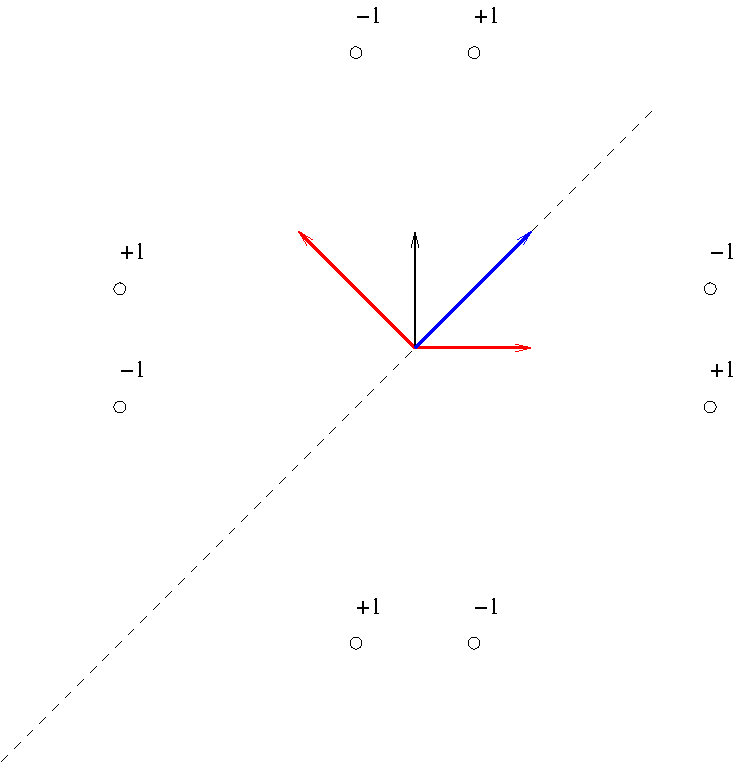
\includegraphics[width=90mm]{B2_A1.pdf}
  }
  \caption{Regular embedding of $A_1$ into $B_2$}
  \label{fig:B2_A1}
\end{figure}
Вот набор аномальных весов $\omega(\mu+\rho)-\rho,\; \omega\in W$ с соответствующими четностями
отражений $\epsilon(\omega)$.
Теперь мы факторизуем группу Вейля $W$ по подгруппе $W_{\bot}=\left\{\omega_1\right\}$. Получаем
следующий набор весов и размерностей представлений  $L^{\pi_{\mathfrak{a}_{\bot}}(\omega(\mu+\rho))-\rho_{\mathfrak{a}_{\bot}}}_{\mathfrak{a}_{\bot}}$:
\begin{figure}[h!tb]
  \noindent\centering{
    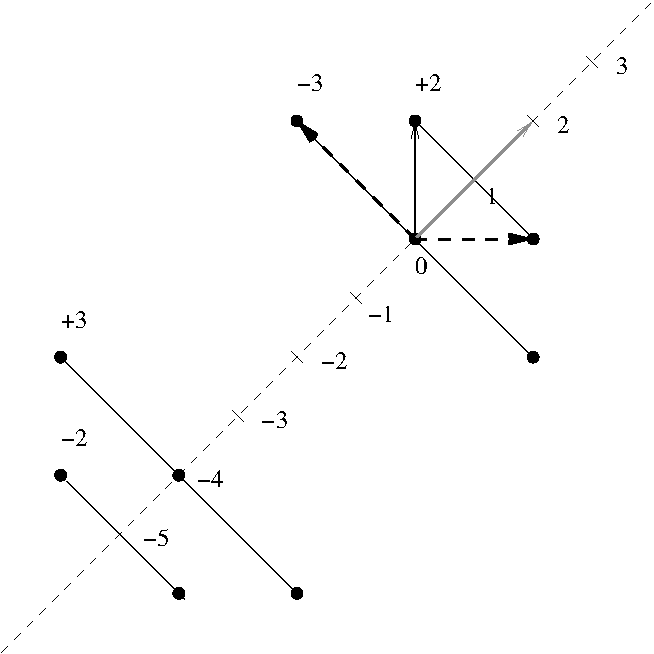
\includegraphics[width=90mm]{B2_A1_2.pdf}
  }
  \caption{Anomalous weights and the corresponding $\mathfrak{a}_{\bot}=A_1$-modules}
  \label{fig:B2_A1_2}
\end{figure}

Затем мы проектируем эти веса и размерности на корневое подпространство подалгебры
$\mathfrak{a}=A_1$ и получаем следующие аномальные веса и их кратности:
\begin{equation}
  \label{eq:25}
  (1,2),\; (0,-3),\; (-4,3),\; (-5,-2)
\end{equation}

Аномальный коэффициент ветвления  $k^{(1,0)}_{1}=2$, для коэффициента $k^{(1,0)}_{0}$ из
рекуррентного соотношения получаем
\begin{equation}
  \label{eq:23}
  k^{(1,0)}_{0}=-1\cdot k^{(1,0)}_2 +2\cdot k^{(1,0)}_1 - 3\cdot \delta_{0,0} = 1
\end{equation}

В работе рассмотрено большое число примеров вложений аффинных алгебр Ли. На самом деле мы написали
программу, которая может строить такие примеры автоматически для алгебр Ли не слишком большого
ранга.

Я сейчас покажу результаты применения нашего алгоритма для одного из примеров конформных вложений.

Рассмотрим такое вложение $\mathfrak{a}\subset \mathfrak{g}$, где
$\mathfrak{a}=\widehat{su(2)}\oplus \widehat{su(2)}$, а $\mathfrak{g}= \widehat{su(4)}$. Это
вложение является аффинным расширением специального вложения конечномерных алгебр Ли $su(2)\oplus
su(2)\subset su(4)$. Это специальное вложение строится следующим образом: берем четырехмерное
представление $su(2)\oplus su(2)$ со старшим весом $(1,1)$. Вот веса этого представления
\ref{fig:A_1+A_1_to_A3}, их координаты в базисе фундаментальных весов: $\nu_1=(1,1),\; \nu_2=(-1,1),\; \nu_3=(1,-1),\; \nu_4=(-1,-1)$.

\begin{figure}[h]
  \begin{multicols}{2}
    \hfill
    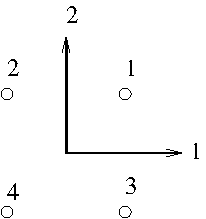
\includegraphics[width=50mm]{A_1+A_1_to_A3.pdf}
    \hfill
    \caption{Representation for the special embedding  $su(2)\oplus su(2)\subset su(4)$}
    \label{fig:A_1+A_1_to_A3}
    \hfill
    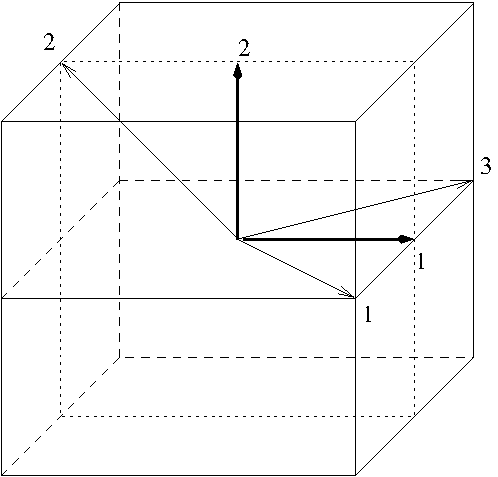
\includegraphics[width=50mm]{A1+A1-A3.pdf}
    \hfill
    \caption{Embedded roots for the special embedding  $su(2)\oplus su(2)\subset su(4)$}
    \label{fig:A1+A1-A3}
  \end{multicols}
\end{figure}

Тогда матричные элементы представления генераторов подалгебры Картана $b_1,b_2$ в базисе Вейля
даются выражениями
$d(b_i)=\mathrm{diag}\left(\frac{2(\nu_1,\alpha_i)}{(\alpha_i,\alpha_i)},\frac{2(\nu_2,\alpha_i)}{(\alpha_i,\alpha_i)},\frac{2(\nu_3,\alpha_i)}{(\alpha_i,\alpha_i)},\frac{2(\nu_4,\alpha_i)}{(\alpha_i,\alpha_i)}\right)$, так что $d(b_1)=\mathrm{diag}(1,-1,1,-1),\;
d(b_2)=\mathrm{diag}(1,1,-1,-1)$.  Отсюда вложенные корни $\alpha_1,\alpha_2$ of $su(2)\oplus su(2)$
выражаются через корни $\tilde{\alpha}_i$ алгебры  $su(4)$
\begin{equation}
  \label{eq:37}
  \begin{array}{l}
     \alpha_1=\frac{1}{2}(\tilde{\alpha}_1+\tilde{\alpha}_3)\\
     \alpha_2=\frac{1}{2}(\tilde{\alpha}_1+2\tilde{\alpha}_2+\tilde{\alpha}_3)
  \end{array}
\end{equation}
Они изображены на рисунке \ref{fig:A1+A1-A3}.

Вложение имеет индексы  $(2,2)$ и является конформным, так как $c(A_1\oplus A_1)=c(A_1)+c(A_1)=2\frac{x_e \mathrm{dim}(A_1)}{x_e+2}=\frac{\mathrm{dim}A_3}{5}=c(A_3)$.

Для построения модулярно-инвариантной статсуммы нам нужно знать редукцию фундаментальных
представлений $\widehat{su(4)}$. Фундаментальные веса имеют следующие координаты в ортогональном базисе
\begin{equation}
  \begin{array}{lll}
     \omega_0 & = & (0,0,0,0;1;0)\\
     \omega_1 & = & (\frac{3}{4},-\frac{1}{4},-\frac{1}{4},-\frac{1}{4}; 1; 0)\\
     \omega_2 & = & (\frac{1}{2},\frac{1}{2},-\frac{1}{2},-\frac{1}{2}; 1; 0)\\
     \omega_3 & = & (\frac{1}{4},\frac{1}{4},\frac{1}{4},-\frac{3}{4}; 1; 0) \\
  \end{array}
\end{equation}


Множества положительных корней  $\Delta^{+}$ и $\Delta_{\mathfrak{a}}^{+}$:
\begin{equation}
  \label{eq:38}
  \begin{array}{lll}
    \Delta^{+} &=&\left\{\co{\Delta}^{+};\; \co{\Delta}-n\delta;\;     -n\delta\;\mbox{with multiplicity}\; 3;\; n=1,2,\dots,\right. \\
    & & \quad\left.\co{\Delta}^{+}=\{\tilde{\alpha}_1, \tilde{\alpha}_2, \tilde{\alpha}_3, \tilde{\alpha}_1+\tilde{\alpha}_2, \tilde{\alpha}_2+\tilde{\alpha}_3, \tilde{\alpha}_1+\tilde{\alpha}_2+\tilde{\alpha}_3\}\right\}\\
    \Delta_{\mathfrak{a}}^{+} &=& \{  \alpha_1,\alpha_2;\;\pm \alpha_1-n\delta,\pm \alpha_2-n\delta;\; -n\delta\; \mbox{with multiplicity} \; 2;\; n=1,2,\dots\}\\
  \end{array}
\end{equation}

Набор $\Delta^{+}_{\bot}$ пуст.
Веер  $\Gamma _{\frak{a}\subset \frak{g}}$ показан на рисунке \ref{fig:A1+A1-A3_fan}. Конечные координаты
даны в базисе фундаментальных весов $su(2)\oplus su(2)$. Элемент $\gamma$ обозначен крестом, если
$s(\gamma)=1$ и кругом, если $s(\gamma)=-1$.
\begin{figure}[h!tb]
  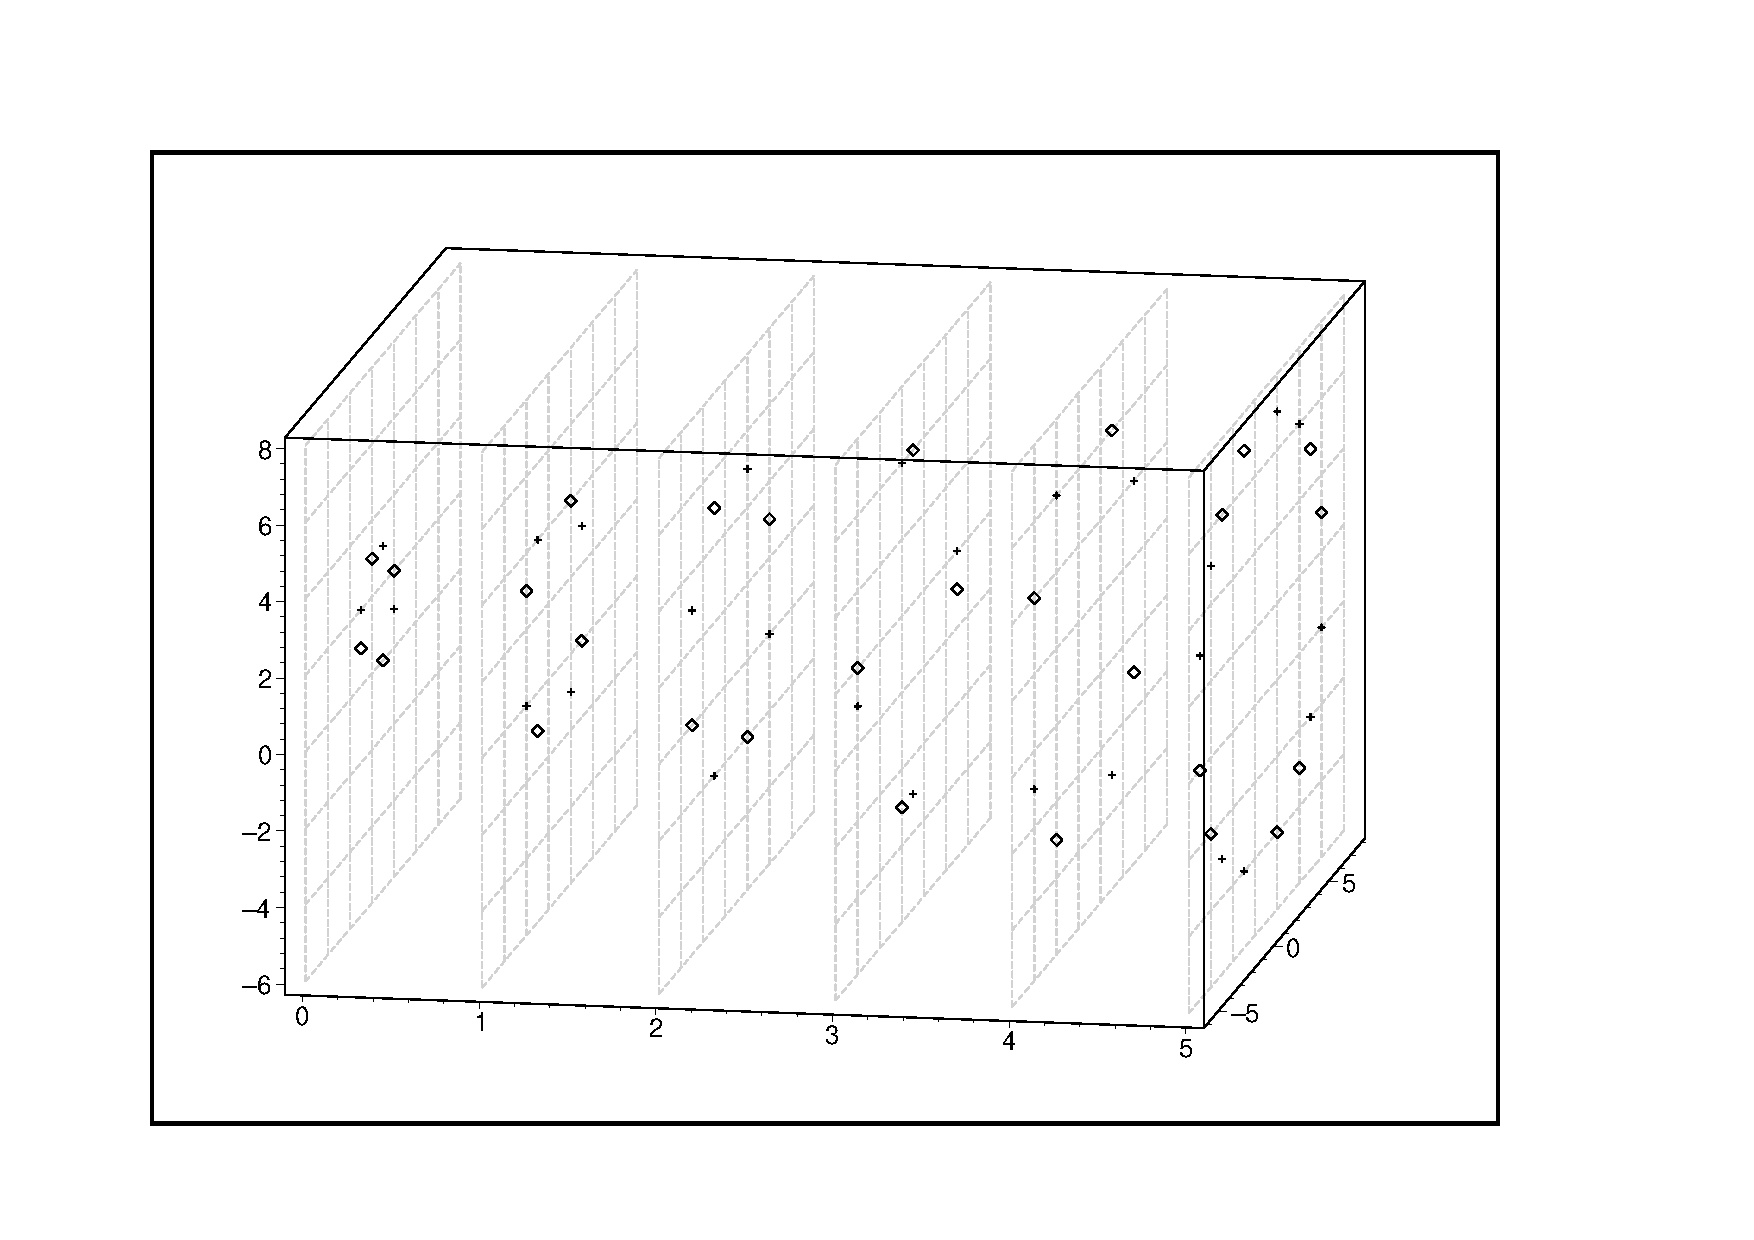
\includegraphics[width=150mm]{A1+A1-A3_fan.pdf}
  \caption{Fan for the special embedding $\widehat{su(2)}\oplus\widehat{su(2)}\subset \widehat{su(4)}$}
  \label{fig:A1+A1-A3_fan}
\end{figure}

Мы ограничимся вычислениями до пятого грейда.
\begin{figure}[h!tb]
  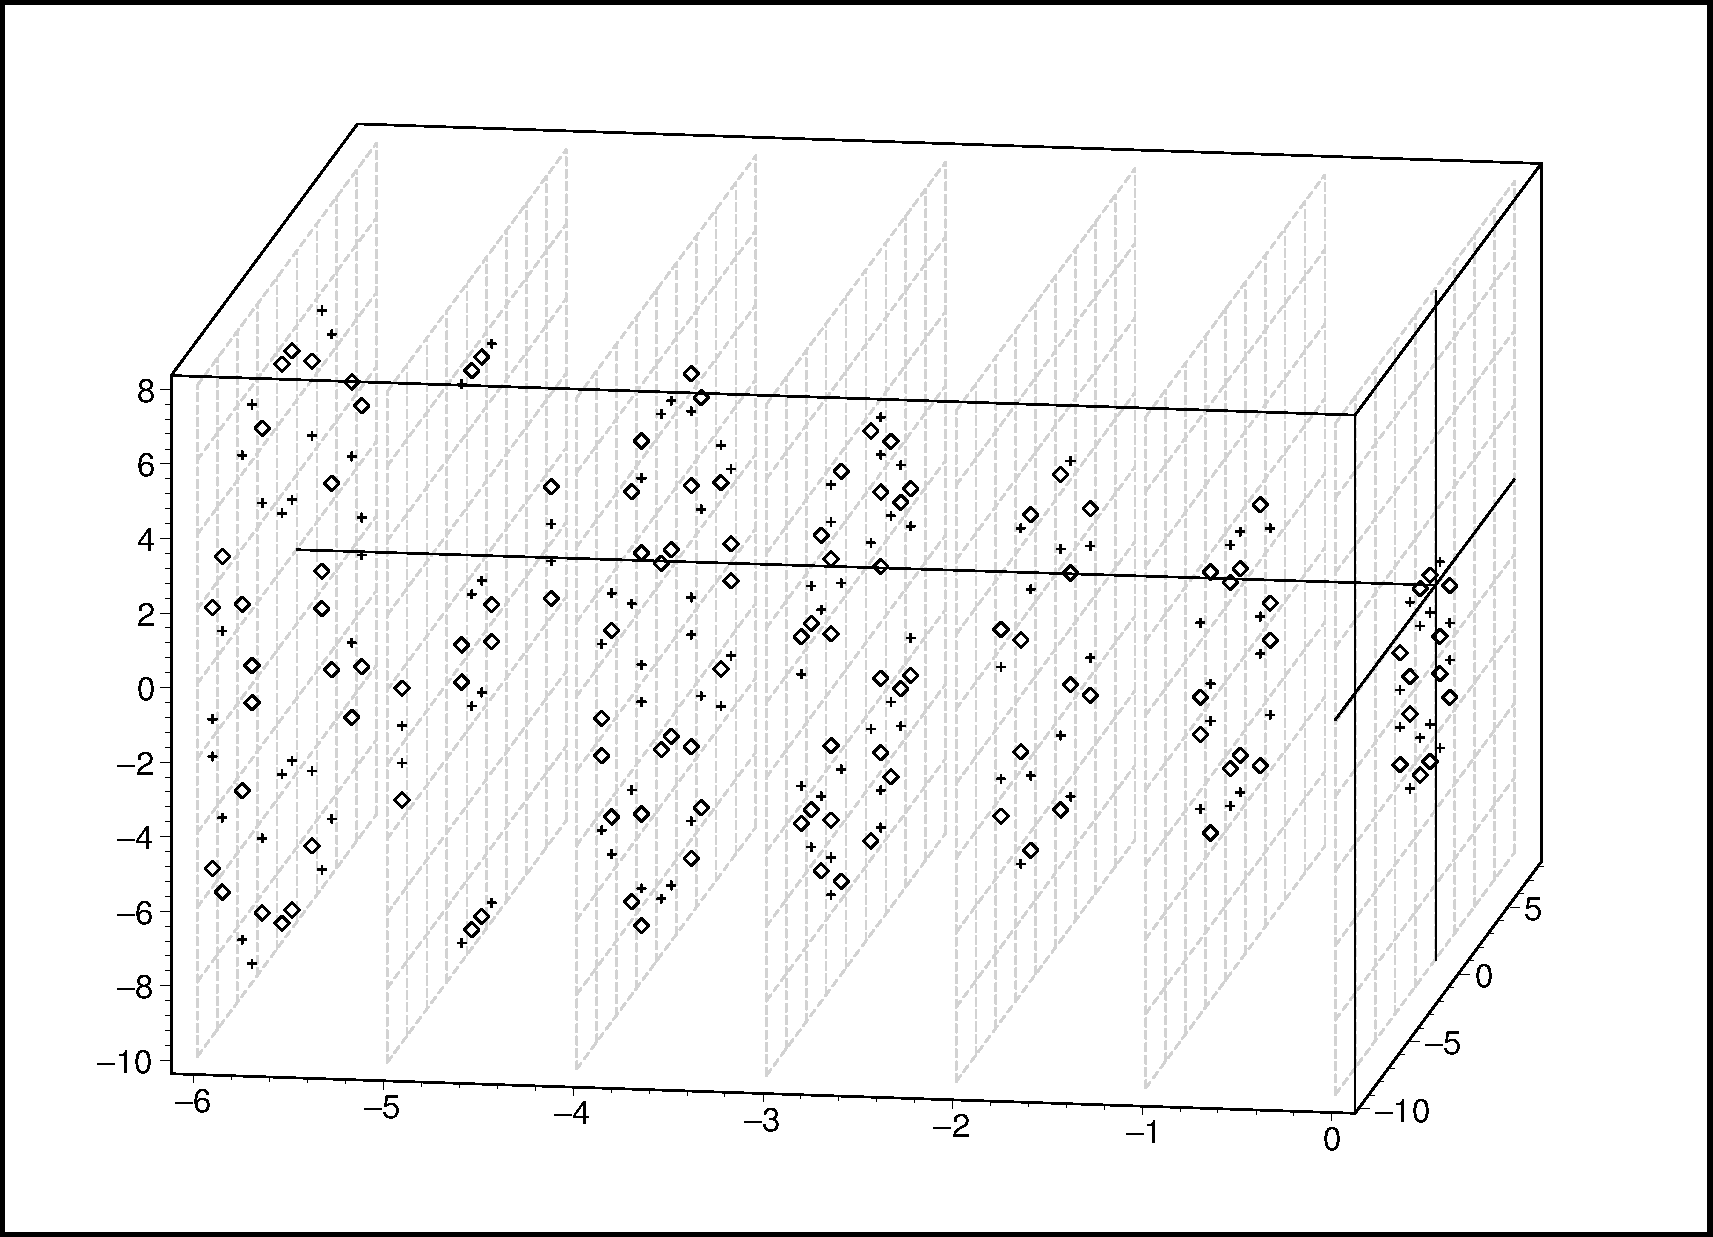
\includegraphics[width=170mm]{A1+A1-A3_anom.pdf}
  \caption{Projected anomalous weights for $L^{\omega_1}_{A_3}$}
  \label{fig:A1+A1-A3_anom}
\end{figure}

Множество аномальных весов  $\widehat{\Psi^{(\mu)}}=\left\{\omega(\mu+\rho)-\rho;\; \omega\in
  W\right\}$ представления алгебры $\hat{A}_3$ состоит из 192 элементов, их проекции
$\pi_{\mathfrak{a}}\left(\widehat{\Psi^{(\mu)}}\right)$ показаны на рисунке  \ref{fig:A1+A1-A3_anom}
для $\mu=\omega_2=(0,0,1;1;0)$.

Аналогичные картинки для $\omega_0, \omega_1,\omega_3$ я не показываю.

Аномальные коэффициенты ветвления для представления  $L^{(\omega_1)}$ вычислены при помощи
рекуррентных соотношений и показаны на рисунке \ref{fig:A1+A1-A3_branching}. 
\begin{figure}[h!tb]
  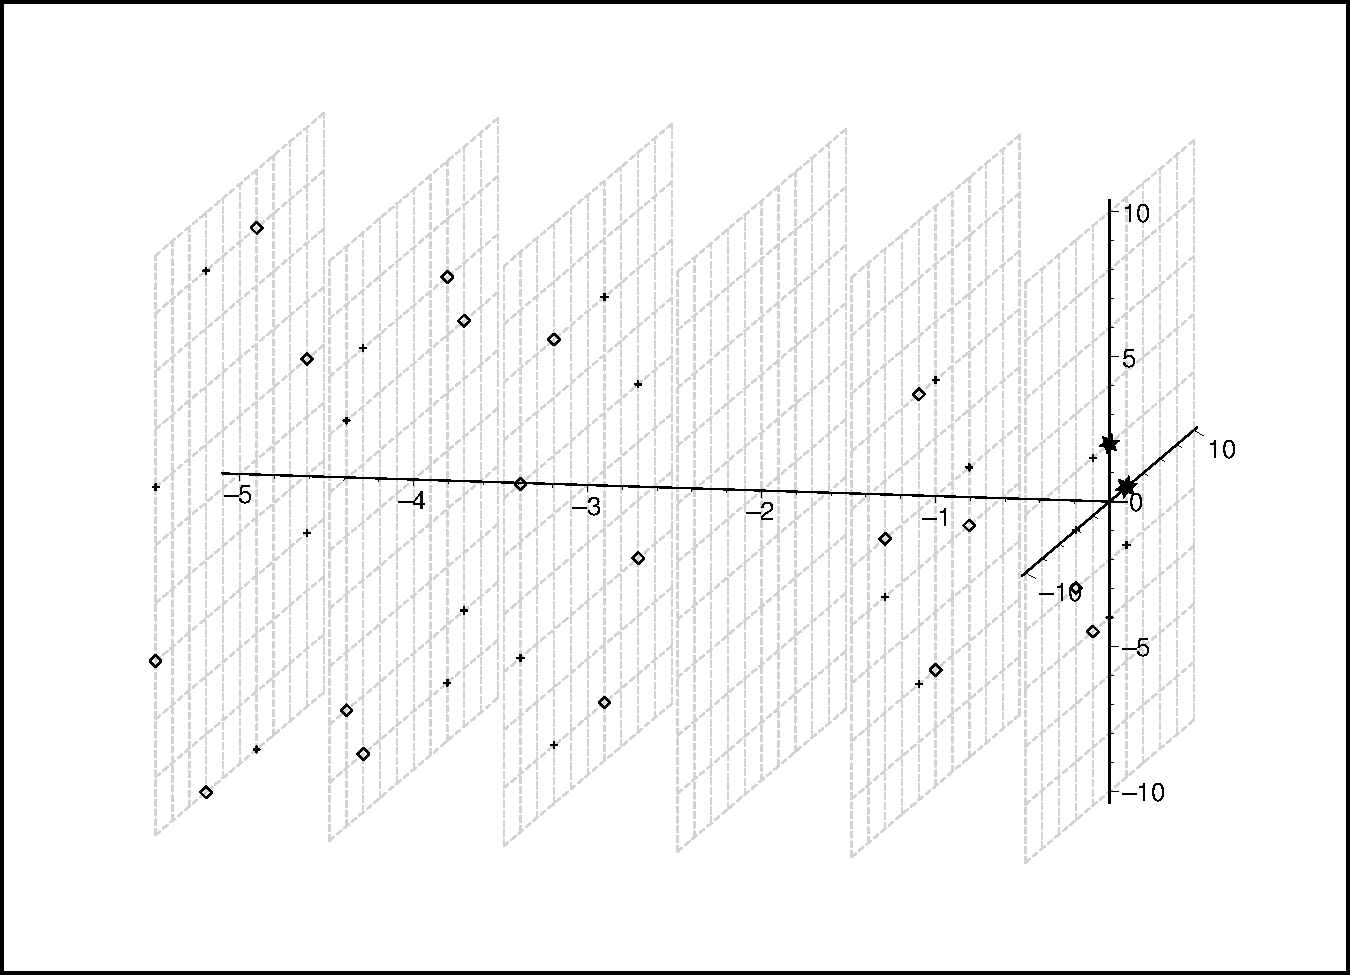
\includegraphics[width=180mm]{A1+A1-A3_branching.pdf}
  \caption{Anomalous branching coefficients for $L^{(0,0,1;1;0)}_{A_3}$}
  \label{fig:A1+A1-A3_branching}
\end{figure}

Получаются следующие правила ветвления:
 \begin{equation}
   \label{eq:39}
   \begin{array}{ll}
     L^{(0,0,0;1;0)}_{\hat{A_3}\downarrow \hat{A_1}\oplus \hat{A_1}}= & L_{\hat{A_1}}^{(0;2;0)}\otimes L_{\hat{A_1}}^{(0;2;0)} \\
     L^{(1,0,0;1;0)}_{\hat{A_3}\downarrow \hat{A_1}\oplus \hat{A_1}}= & L_{\hat{A_1}}^{(1;2;0)}\otimes L_{\hat{A_1}}^{(1;2;0)} \\
     L^{(0,1,0;1;0]}_{\hat{A_3}\downarrow \hat{A_1}\oplus \hat{A_1}}= & \left( L_{\hat{A_1}}^{(2;2;0)}\otimes L_{\hat{A_1}}^{(0;2;0)}\right) \oplus \left( L_{\hat{A_1}}^{(0;2;0)}\otimes L_{\hat{A_1}}^{(2;2;0)}\right) \\
     L^{(0,0,1;1;0)}_{\hat{A_3}\downarrow \hat{A_1}\oplus \hat{A_1}}= & L_{\hat{A_1}}^{(1;2;0)}\otimes L_{\hat{A_1}}^{(1;2;0)} \\     
   \end{array}
 \end{equation}

В результате мы получаем модулярно-инвариантную статсумму для WZW-модели с киральной алгеброй $\hat{A}_1\oplus \hat{A}_1$.
\begin{multline}
  \label{eq:40}
  Z=\left|\chi_{(0;2;0)}\chi_{(0;2;0)}\right|^2+2\left|\chi_{(1;2;0)}\chi_{(1;2;0)}\right|^2+ \left|\chi_{(2;2;0)}\chi_{(0;2;0)}+\chi_{(0;2;0)}\chi_{(2;2;0)}\right|^2=\\
  \left|\chi_{(0;2;0)}\right|^4+2\left|\chi_{(1;2;0)}\right|^4+ 4\left|\chi_{(2;2;0)}\chi_{(0;2;0)}\right|^2
\end{multline}

\section{Заключение. Обсуждение перспектив.}
\label{sec:conlusion}

Недавно мы заметили, что струнные функции, которые описывают представления, модулярные функции,
которые описывают редукцию представлений и функции слияния, которые описывают разложение тензорных
произведений представлений на неприводимые, допускают построение дуальных систем функций. Эти
дуальные функции могут быть построены просто из анализа соответствующих групп Вейля, при этом многие
известные результаты могут быть перенесены на них, например, результаты Каца о модулярных свойствах
струнных функций и функций ветвления. И наоборот. 

В настоящее время мы начали исследовать эти системы дуальных функций. 

Среди других возможных приложений полученных методов можно отметить также приложения в интегрируемых
цепочках, а также в приложения дуальных функций теории модулярных форм. 

\section{Замечания}
\label{sec:notes}

1. Модулярную инвариантность рассказать удовлетворительно не удастся,
и по времени тоже не удастся. Следовательно, её кратко помянуть и
постулировать выражение (46). Все, что до стр 10, рассказать.
Слушатель должен быть убежден в том, что модули афф. алгебры
фигурируют в искомом выражении.
2. Нуждается в обосновании сама постановка вопроса о редукции в
этих теориях. Иначе появление подалгебры ничем не обосновано.
3. Необходимо сказать об общей идеологии веера вложений.
Ведь дотошно объяснить все на примере формулы (53) вряд ли
возможно. Значит надо объяснить идею.


Мелкие замечания:
1.стр.1
"Наша задача   придумать практический алгоритм
вычисления коэффициентов этого разложения."

Придется 2 слова сказать о том, что мы не первые
решаем эту задачу, мы решаем её новыми методами,
эффективность таких методов выше и т.п.

2.стр.2
"В этом случае конформная группа   это набор всех ана-
литических функций w(z) на плоскости."

Как это понимать?

3.стр.3
"Все поля в теории оказываются суммами мультиплетов алгебры Вирасо-
ро."

Все поля в теории вполне приводимы и разлагаются в прямую сумму
подпространств, инвариантных относительно алгебры Вирасо-
ро.

4.стр.3
Про "аномальные размерности" ничего не было сказано.

5.стр.
"Он определен на трехмерном многообразии B, ограниченном исходным
двумерным пространством."
Это должно быть сказано в начале параграфа.

6.стр.4
"Разность значений члена Весса-
Зумино на этих многообразиях дается правой частью уравнения (10)
с интегралом, продолженным на все компактное трехмерное простран-
ство."

Осталось неясно, может нарисовать?

7.стр.5
"для полного действия (42):"

Уж наверное не 42, а 8?

8.стр.6

формулы (30) и (31) непонятны.

9.стр.
"hv - дуальное число Кокстера."

Дать явное выражение.

10.стр.7
"бесконечномерные и неинтегрируемые поля отщепляют-
ся в корреляционных функциях."

Что это значит?

11.
"Представления алгебры можно рас-
сматривать как сумму представлений подалгебры."

Откуда взялась подалгебра?


\end{document}


